%!TEX root = ../colloquium.tex

\begin{frame}[plain,noframenumbering]
	\centering
	\vspace*{2.6cm}
	\Huge{\colorit{Part III}}\\
%	{\large(time-permitting)}
	\vskip 20pt
	\Large{Hyperharmonic analysis}
\end{frame}

\begin{frame}{Graph Laplacian}
	\pause
	Given a function $\phi$ on the vertices of a weighted graph
	\[
	\Delta\phi(v) = \sum_{[u,v]} \gamma_{[u,v]}(\phi(v) - \phi(u))
	\]
	where $\gamma_{[u,v]}$ is the weight of $[u,v]$.

	\pause\bigskip
	\colorit{Remark:} It is an approximation to the (smooth) Laplace operator.

	\pause\bigskip
	This an other versions are used for:

	\smallskip
	\colorit{Clustering analysis},

	\colorit{Dimensionality reduction},

	\colorit{Random walk analysis},

	\colorit{Image and signal processing},

	\vspace*{-3pt}
	$\qquad\qquad \colorit{\vdots}$

	\pause\medskip

	Is there an analogue for \colorit{simplicial complexes}?
\end{frame}

\begin{frame}{Discrete Laplacian}
	\pause
	Given a weighted simplicial complex and a function $\phi$ on its $n$-simplices
	\[
	\Delta_n\phi = (\bd_{n+1} \delta_n + \delta_{n-1} \bd_n)\phi,
	\]
	where $\bd$ is the boundary operator and $\delta$ its adjoint with respect to the inner product defined by the weights.

	\pause\bigskip
	\colorit{Remark:} It is an approximation to the (smooth) Laplace--Beltrami operator of Riemannian geometry.

	\pause\bigskip
	\colorit{Remark:} Connection with topology
	\[
	\dim(\ker \Delta_n) = \beta_n.
	\]

	\pause\medskip
	We will use it for signal processing.

	\pause\medskip
	First, let us introduce examples of functions on higher simplices.
\end{frame}

\begin{frame}{Information signals}
	\pause
	Let $X_0, \dots, X_N$ be probability distributions

	\vskip 5pt

	\begin{itemize}
		\pause\item The \colorit{entropy} of each
		\[
		\textstyle H(X_i) = - \sum_{x_i} p(x_i) \log p(x_i).
		\]
		\vspace*{-20pt}\pause\item The \colorit{mutual information} of pairs
		\[
		I(X; Y) = H(X, Y) - H(X \mid Y) - H(Y \mid X).
		\]
		\vspace*{-20pt}\pause\item The \colorit{interaction information} of triples
		\begin{align*}
			I(X;Y;Z) &=
			H(X) + H(Y) + H(Z) \\
			& - H(X,Y) - H(X,Z) - H(Y,Z) \\
			& + H(X,Y,Z).
		\end{align*}
		\vspace*{-20pt}\pause\item \colorit{Analogues} for higher cardinality subsets.
	\end{itemize}

	\pause\smallskip

	\colorit{Problem:} Number of subsets \colorit{grows exponentially} with $N$.

	\smallskip
	\colorit{Question:} Can we compress these signals?
\end{frame}

\begin{frame}{Hyperharmonic analysis}
	\pause
	\colorit{Fourier basis:} Eigenvectors of the discrete Laplacian.

	\pause\bigskip
	\colorit{Contribution (Med.--Rosas--Rodr\'iguez--Cofr\'e)}\\
	Compression of higher-order information signals using the Fourier basis.

	\pause\bigskip
	\colorit{Analogy:} Listen to a few harmonics to tell a guitar and a~piano apart.

	\pause\bigskip
	How to measure \colorit{compressibility}?

	\pause\bigskip
	Give signal $\alpha$, let $\{\alpha_i\}$ be its coeff's in a basis with $\alpha_1^2 \geq \alpha_2^2 \geq \cdots$
	\begin{equation*}
		\text{EV}_{\alpha}(k) = \frac{ \alpha_k^2}{{\displaystyle \sum_{i} \alpha_i^2}}
		\qquad \text{ and } \qquad
		\text{CEV}_{\alpha}(k) = \sum_{1\leq i \leq k} \text{EV}_{\alpha}(i),
	\end{equation*}
\end{frame}

\begin{frame}{Proof of concept: Haydn's symphonies}
	\pause\vskip -5pt
	Music as a probability distribution.

	\pause\vskip 5pt
	We analyzed two high-order information signals across four dimensions:

	\pause\vskip 7pt
	\hspace*{-15pt}
	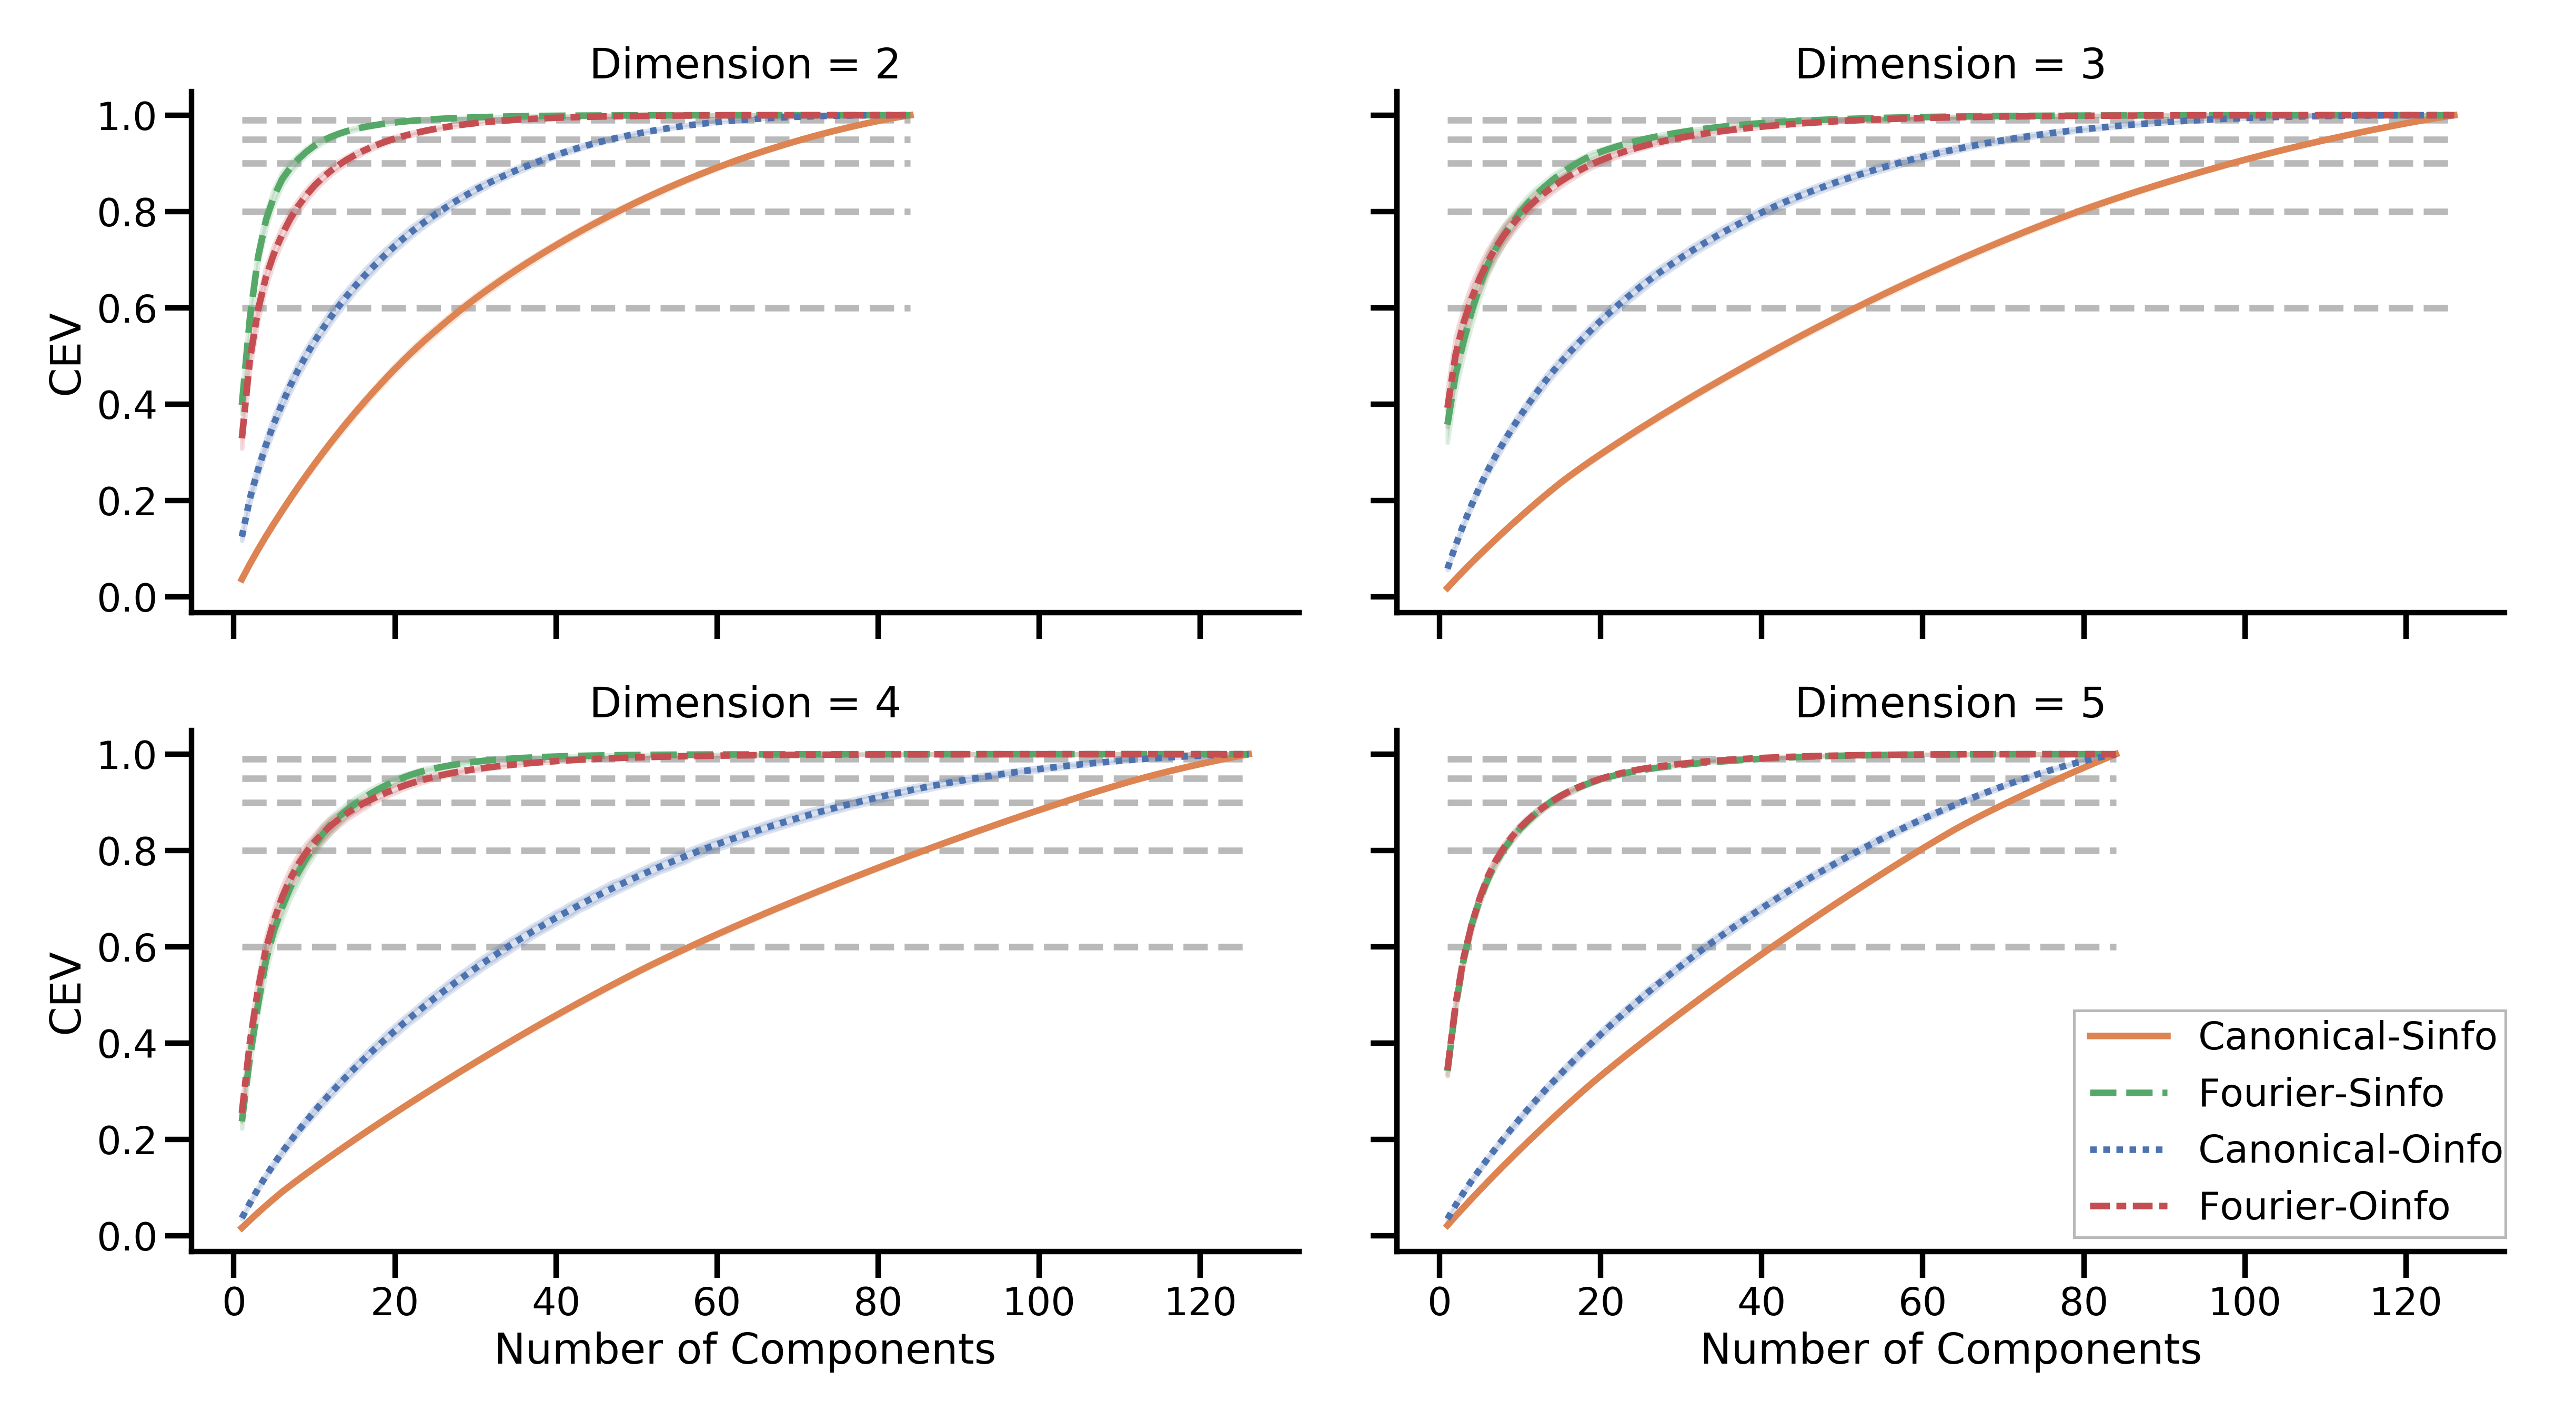
\includegraphics[scale=.096]{aux/hyperharmonic}
\end{frame}

\begin{frame}{Summary: Signal processing on hypergraphs}
	\colorit{Case study:} Compressing high-order information signals.

	\pause\medskip
	\begin{itemize}
		\itemsep15pt % Adjusts the space between items
		\item Higher order information signals capture interactions between multiple nodes of a system.

		\item The dimension of these signals grows exponentially with the number of nodes.

		\item The eigenvectors of the discrete Laplacian provide a new basis.

		\item A few Fourier vectors carry most of the signal.
	\end{itemize}
\end{frame}